% Technical report: Assignment 4, Edge Computing & Intelligent Systems.
% Build:  python scripts/make_report_assets.py && cd docs/report && pdflatex report && pdflatex report
\documentclass[10pt,a4paper]{article}

\usepackage[margin=1.8cm,top=1.6cm,bottom=1.8cm]{geometry}
\usepackage{lmodern}
\usepackage[T1]{fontenc}
\usepackage{amsmath,amssymb}
\usepackage{graphicx}
\usepackage{array,tabularx}
\usepackage{color}
\usepackage{url}
\usepackage{fancyhdr}
\usepackage[hidelinks]{hyperref}

% ---------------------------------------------------------------- student details (edit)
\newcommand{\studentname}{Your Name}
\newcommand{\rollno}{22i-0000}
\newcommand{\sectionid}{A}
\makeatletter
\renewcommand\section{\@startsection{section}{1}{\z@}{-2.2ex \@plus -1ex \@minus -.2ex}%
  {1.0ex \@plus .2ex}{\normalfont\large\bfseries}}
\renewcommand\subsection{\@startsection{subsection}{2}{\z@}{-1.6ex\@plus -1ex \@minus -.2ex}%
  {0.6ex \@plus .2ex}{\normalfont\normalsize\bfseries}}
\makeatother

% booktabs-style rules without booktabs
\newcommand{\toprule}{\noalign{\hrule height 0.8pt}}
\newcommand{\midrule}{\noalign{\hrule height 0.4pt}}
\newcommand{\bottomrule}{\noalign{\hrule height 0.8pt}}
\renewcommand{\arraystretch}{1.12}
\setlength{\tabcolsep}{4pt}
\setlength{\parskip}{2pt}
\setlength{\textfloatsep}{8pt plus 2pt}
\setlength{\floatsep}{6pt plus 2pt}
\setlength{\abovecaptionskip}{3pt}
\setlength{\belowcaptionskip}{3pt}

\definecolor{accent}{rgb}{0.62,0.18,0.14}   % dark red; no blue anywhere
\newcommand{\code}[1]{\texttt{\small #1}}
% primitive \input is expandable, so generated rows can sit before \noalign rules
\newcommand{\tabinput}[1]{\csname @@input\endcsname #1 }

\pagestyle{fancy}
\fancyhf{}
\lhead{\small Edge Computing \& Intelligent Systems --- Assignment 4}
\rhead{\small \rollno\ (\sectionid)}
\cfoot{\small \thepage}
\renewcommand{\headrulewidth}{0.4pt}

\begin{document}

\begin{center}
  {\LARGE\bfseries Knowledge Distillation and Hardware-Aware NAS for Edge Deployment}\\[4pt]
  {\large \studentname\ \quad \rollno\ \quad Section \sectionid}\\[2pt]
  {\small Code, checkpoints and results: \url{https://github.com/guzorpazorp/edge_compute_assignment_4}}
\end{center}
\vspace{-4pt}
\noindent\textcolor{accent}{\rule{\linewidth}{0.8pt}}

\section{Overview}
The project is a single repository with one script per pipeline step. Every step reads the outputs
of the previous one by naming convention (\code{checkpoints/<run>/best.pt},
\code{results/...}), so no paths need to be edited by hand. All hyper-parameters live in
\code{configs/\{teacher,student,nas\}.yaml}, and any of them can be overridden from the command line with
\code{-{}-set key=value}. Work was split across machines according to its cost:

\begin{center}\small\setlength{\tabcolsep}{3.5pt}
\begin{tabular}{llll}
\toprule
Step & Script & Hardware & Wall time \\
\midrule
Teacher ResNet-50 (30 ep.) & \code{train\_teacher.py} & Colab T4 & 34.7 min \\
3 baselines / 3 KD students (20 ep.) & \code{train\_student.py} & Colab T4 & 23.7 / 34.3 min \\
NAS search (40 trials) + retrain (20 ep.) & \code{nas\_search.py}, \code{nas\_retrain.py} & GTX 1060 & $\sim$25 + 4.6 min \\
ONNX export, inference, benchmark & \code{export\_onnx.py}, \code{infer.py}, \code{benchmark.py} & i7-8665U (CPU) & minutes \\
\bottomrule
\end{tabular}
\end{center}
Training saves a per-epoch \code{last.pt} (full state, for resuming after a Colab disconnect), a
weights-only \code{best.pt} that also carries metadata (architecture, classes, resolution, config),
and a CSV log per run.

\section{Question 1: Knowledge Distillation on CIFAR-100}

\subsection{Teacher and students}
\textbf{Teacher.} \code{src/models/resnet.py} implements ResNet-50 from scratch. Its parameter names
mirror torchvision's, so the model is initialised from ImageNet-1k weights and fine-tuned; only the
100-way classifier is new. For $32{\times}32$ inputs the $7{\times}7$ stem keeps its weights but uses
stride 1, and the max-pool is removed, so \code{layer1} still sees $32{\times}32$ maps. Training ran
for 30 epochs: SGD with Nesterov momentum, learning rate 0.05 with the backbone at 0.2$\times$,
cosine schedule, mixed precision. The teacher reaches \textbf{86.74\%} top-1. Fine-tuning gives a
strong teacher (the quality of the soft targets bounds what KD can transfer) at a fraction of the
$\sim$200 epochs needed from scratch. The \emph{students are never pretrained}, so the baseline-vs-KD
comparison isolates the effect of distillation.

\textbf{Students} (\code{src/models/}) are written from the papers and adapted to CIFAR by removing
early down-sampling, which leaves a final feature map of $4{\times}4$:
MobileNetV2 (inverted residuals, 2.35\,M parameters);
SqueezeNet\,1.1 (Fire modules, 0.78\,M), with BatchNorm added inside the Fire modules and the ReLU on the logits
removed, because non-negative logits distort the softmax;
and EfficientNet-Lite0 (3.50\,M), which is B0 without squeeze-and-excitation, uses ReLU6, and has a fixed
stem and head. Every model implements \code{forward(x, return\_feats=True)}, which also returns its
$8{\times}8$ intermediate feature map for feature distillation.

\subsection{Distillation framework}
\code{src/kd/distill.py} implements the loss
\begin{equation}
\mathcal{L} = \alpha\,T^2\,\mathrm{KL}\!\left(\sigma(z_t/T)\,\|\,\sigma(z_s/T)\right)
 + (1-\alpha)\,\mathrm{CE}(z_s, y)
 + \beta\,\big\|\,n(A(f_s)) - n(f_t)\,\big\|_2^2 ,
\end{equation}
which covers all four required features. The first term is \emph{soft-target KD} with a
\emph{temperature softmax}; the $T^2$ factor keeps its gradients on the same scale as the CE
term. Together with the CE term it gives \emph{combined hard- and soft-label training}. The third
term is \emph{feature-based distillation} (FitNets): the teacher's \code{layer3} map $f_t$ (1024 channels,
$8{\times}8$) is the hint, and a $1{\times}1$ conv + BN adapter $A$ projects the student's $8{\times}8$
stage onto it. Both maps are L2-normalised per sample ($n$). Without this normalisation the term was
$\approx$90 at initialisation and dominated the loss. Defaults: $T{=}4$, $\alpha{=}0.9$, $\beta{=}5$.
Each term can be switched on or off in \code{student.yaml}. All three students train
\emph{jointly} on the same batches: one frozen fp16 teacher forward pass serves all of them, which
removes two-thirds of the teacher compute. Baselines use the same script and schedule with
\code{-{}-mode baseline}, which trains with CE only. Students use 20 epochs, batch 128, learning rate 0.05,
cosine schedule and mixed precision.

\subsection{Results}
\begin{figure}[h]
  \centering
  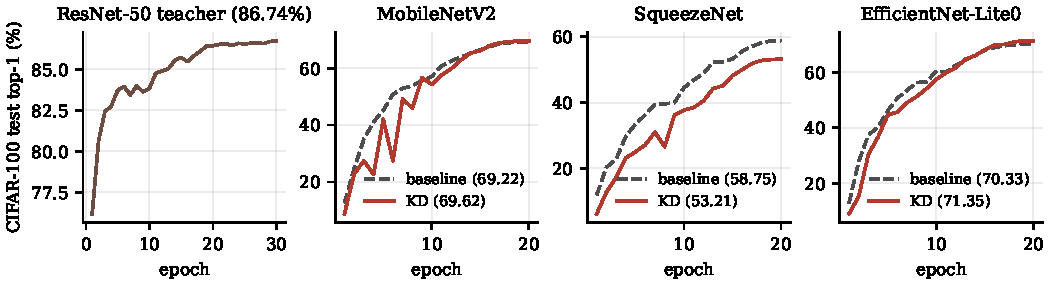
\includegraphics[width=\linewidth]{figs/q1_curves.pdf}
  \caption{CIFAR-100 test accuracy per epoch: the teacher, and each student trained with and without KD.}
  \label{fig:q1}
\end{figure}

\begin{table}[h]\centering\small
\caption{Best CIFAR-100 test accuracy (\%). The KD gain is measured against the student's own baseline, with identical schedule and seed.}
\label{tab:q1}
\begin{tabular}{lrrrrrr}
\toprule
Model & Params & Baseline top-1 & KD top-1 & $\Delta$ top-1 & Baseline top-5 & KD top-5 \\
\midrule
ResNet-50 teacher & 23.71\,M & 86.74 & -- & -- & 98.15 & -- \\
MobileNetV2 & 2.35\,M & 69.22 & 69.62 & +0.40 & 91.51 & 92.33 \\
SqueezeNet & 0.78\,M & 58.75 & 53.21 & $-$5.54 & 86.05 & 82.71 \\
EfficientNet-Lite0 & 3.50\,M & 70.33 & \textbf{71.35} & \textbf{+1.02} & 91.75 & 92.85 \\
\bottomrule
\end{tabular}
\end{table}

\textbf{Discussion.} KD improves the two larger students in both top-1 and top-5 (+0.8 and +1.1 top-5).
Their train/test gap is also smaller: train accuracy is 81--85\% with KD against 85--90\% without, which
is consistent with soft targets acting as a regulariser. The gains are modest because each student
had only 20 epochs, and KD usually pays off more over longer schedules. \textbf{SqueezeNet gets worse
with KD}, and its training accuracy also falls (56\% vs.\ 65\%), so this is under-fitting rather than
over-fitting. Three causes combine. (i) A large capacity gap: SqueezeNet has 30$\times$ fewer
parameters than the teacher. (ii) With $\alpha{=}0.9$ the hard labels carry only 10\% of the
loss, and the feature hint forces SqueezeNet's 256-channel stage to imitate a 1024-channel map, which
uses up capacity it needs for classification. (iii) The schedule is short, and its KD loss is
still falling at epoch 20. The usual fixes are a lower $\alpha$, dropping the feature term, or a teacher
assistant. We report the result as observed. The early oscillation of the KD MobileNetV2 curve
(Fig.~\ref{fig:q1}) disappears once the learning rate decays.

\subsection{Unified inference and ONNX deployment}
\code{src/deploy/runtime.py} defines one \code{Predictor(run, backend)} class for every model,
with backend \code{torch} or \code{onnx}. It rebuilds preprocessing (resize, normalise) and the class
names from the checkpoint metadata, or from a JSON sidecar next to the \code{.onnx} file, so ONNX
Runtime inference needs no PyTorch model code. \code{scripts/infer.py} classifies a single image or
evaluates the test set, with either backend or both side by side. \code{scripts/export\_onnx.py}
exports every model (opset 17, dynamic batch) and checks parity against PyTorch. The maximum absolute
logit difference was at most $6.4{\times}10^{-6}$ for all models, and on the full 10\,000-image test sets
the PyTorch and ONNX Runtime accuracies matched to two decimals for every model (Fig.~\ref{fig:console}).

\section{Question 2: Hardware-Aware NAS on CIFAR-10}

\subsection{Search space and generator}
An architecture is a JSON dictionary (\code{src/nas/space.py}). The search space covers every
required dimension:
\begin{center}\small
\begin{tabular}{ll}
\toprule
Dimension & Choices \\
\midrule
Depth & 2--4 stages (strides 1,2,2,2) $\times$ 1--3 blocks per stage \\
Channels & stem $\{16,24,32\}$; per stage $\{16,24,32\}$, $\{32,48,64\}$, $\{64,96,128\}$, $\{128,160,256\}$; head $\{0,256,512\}$ \\
Kernel size & $\{3,5,7\}$ per stage \\
Block type & standard conv--BN--act, or depthwise-separable (dw $k{\times}k$ $\to$ pw $1{\times}1$) \\
Activation & ReLU, ReLU6, Hard-Swish, SiLU (per stage) \\
Input resolution & $\{24, 32, 40\}$ \\
\bottomrule
\end{tabular}
\end{center}
\code{src/nas/builder.py} turns a sampled configuration into an \code{nn.Module}, using the modules
\code{ConvBlock}, \code{DWSepBlock} and \code{NASNet}. A residual connection is added when a block's
shape is preserved, followed by global pooling and a linear classifier.

\subsection{Search strategy and hardware-aware selection}
The search uses Bayesian optimisation with \textbf{Optuna TPE}: 8 random start-up trials, then 32 TPE
trials, plus a \code{MedianPruner}. The study is stored in SQLite, so the search resumes after an
interruption. Each trial (\code{src/nas/search.py}) runs these steps:
\begin{enumerate}\itemsep0pt
  \item Sample and build the architecture.
  \item \textbf{Profile it on the CPU before any training} (\code{src/nas/hw\_profile.py}):
  median batch-1 latency over 30 runs with 1 thread; storage size of the serialised fp32
  \code{state\_dict}; peak inference memory from the PyTorch profiler's allocation events plus the
  weights; parameter count and FLOPs.
  \item \textbf{Reject} the trial if it violates a deployment constraint (latency $\le$ 3\,ms,
  size $\le$ 1\,MB, peak memory $\le$ 12\,MB). The trial is recorded with accuracy 0 and the reason,
  so TPE learns to avoid that region and no GPU time is spent on it.
  \item Otherwise, proxy-train it for 4 epochs on a 20k-image subset and validate on a 5k split held
  out from the training set (the test set is never used in the search). The data stays in GPU memory
  and is augmented on the GPU, because tiny CNNs are otherwise limited by data loading.
  \item Architectures that TPE proposes again reuse their earlier result, so latency noise cannot
  flip a verdict.
\end{enumerate}
After every trial the complete history is written to \code{results/nas/history.\{csv,json\}} and the
best feasible architecture to \code{best\_arch.json}. \code{nas\_retrain.py} then trains that
architecture from scratch on all 50\,000 images. The constraint thresholds were calibrated by
profiling random architectures on the laptop, so that about 70\% of samples pass.

\subsection{Results}
\begin{figure}[h]
  \centering
  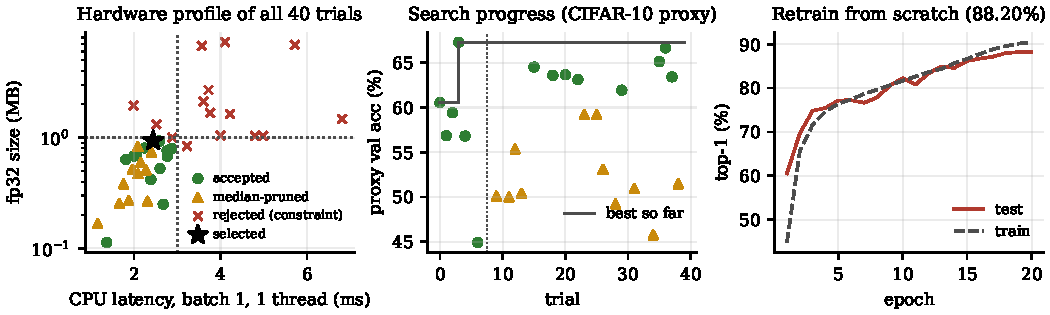
\includegraphics[width=\linewidth]{figs/nas.pdf}
  \caption{Left: latency and size of all 40 trials; dotted lines mark the constraints. Middle: proxy
  validation accuracy of trained candidates (rejected trials are not trained; the dotted line ends the 8 random start-up trials). Right: training curves of
  the selected architecture, retrained from scratch.}
  \label{fig:nas}
\end{figure}
Of the 40 trials, \textbf{15 were rejected} by the hardware check. 14 broke the size limit, 12 the latency
limit and 3 the memory limit; most rejected trials broke more than one. A further \textbf{11 were
median-pruned} and \textbf{14 completed} (Fig.~\ref{fig:nas}). TPE converged on one region of the space:
input resolution 40, a narrow stem (16 channels), cheap standard convolutions at high
resolution, and depthwise-separable $7{\times}7$ blocks in the last stage, where large kernels are cheap.
\emph{Size was the binding constraint}: the top three candidates all sit at 0.93\,MB, just under the
1\,MB limit.
\begin{table}[h]\centering\small
\caption{Top-5 completed candidates (latency profiled on the search machine, a Xeon E3-1220 v3).}
\label{tab:nastop}
\begin{tabularx}{\linewidth}{rrrrrr>{\raggedright\arraybackslash}X}
\toprule
Trial & Val acc & Params & Size (MB) & Lat.\ (ms) & Mem (MB) & Architecture \\
\midrule
\tabinput{tables/nas_top.tex}
\bottomrule
\end{tabularx}
\end{table}

The selected architecture (trial 3) has 236k parameters and 69.9 MFLOPs. Retrained from scratch for
20 epochs (4.6\,min on the GTX 1060), it reaches \textbf{88.20\%} CIFAR-10 test top-1, or 88.00\% through
the ONNX Runtime inference pipeline, which uses a different resize path. It was exported to
\code{onnx/nas\_best.onnx} (0.91\,MB) and runs through the same \code{Predictor} and \code{infer.py} as
the Q1 students.

\section{Benchmarking}
\code{scripts/benchmark.py} benchmarks every available model on the deployment laptop (Intel i7-8665U,
1 thread, batch 1). For each model it records parameters, FLOPs, checkpoint and ONNX size, median
PyTorch and ONNX Runtime latency over 100 runs, peak inference memory, and test accuracy through
ONNX Runtime. The results go to \code{results/benchmark.csv} (Table~\ref{tab:bench}).

\begin{table}[h]\centering\small
\caption{Benchmark on the deployment CPU (i7-8665U, 1 thread, batch 1). C-100 = CIFAR-100, C-10 = CIFAR-10.
Sizes are fp32 checkpoint / ONNX file sizes in MB; latency is in ms; peak memory is in MB.}
\label{tab:bench}
\begin{tabular}{lcrrrrrrrr}
\toprule
Model & Data & Params (M) & MFLOPs & Size & ONNX & Torch lat. & ORT lat. & Peak mem & Top-1 \\
\midrule
\tabinput{tables/benchmark.tex}
\bottomrule
\end{tabular}
\end{table}

\textbf{Observations.} (i) \emph{ONNX Runtime is 1.2--6.6$\times$ faster than eager PyTorch} on the
same CPU and thread count, because of graph-level fusion (Conv+BN+activation) and lower per-operator
overhead. The gain is largest for small networks, where that overhead dominates.
(ii) The \emph{NAS model is the only model that meets all three deployment constraints (latency, size, memory), and it does so on the deployment laptop too}:
1.95\,ms in PyTorch and 0.85\,ms in ONNX Runtime, against the 3\,ms limit set during the search.
This i7 is faster per thread than the Xeon used during the search (2.44\,ms). The NAS model is also the
smallest (0.93\,MB, 6.6\,MB peak memory). Its accuracy is on CIFAR-10, so it cannot be compared
directly with the CIFAR-100 students.
(iii) Among the students, EfficientNet-Lite0 with KD has the best accuracy but is the largest and slowest.
SqueezeNet is 3--8$\times$ cheaper but loses 11--18 points.
(iv) A baseline and its KD counterpart have the same architecture, so their latency differences
(e.g.\ SqueezeNet 0.56 vs.\ 1.24\,ms) are measurement noise on a laptop CPU with turbo boost, not a property
of the models.

\begin{figure}[h]
\centering
\begin{minipage}{0.97\linewidth}
\scriptsize
\begin{verbatim}
$ python scripts/export_onnx.py --include-teacher
[kd_mbv2] -> kd_mbv2.onnx  (8.95 MB)  parity max|diff|=1.91e-06 OK
[kd_efflite0] -> kd_efflite0.onnx  (13.31 MB)  parity max|diff|=2.62e-06 OK
[nas_best] -> nas_best.onnx  (0.91 MB)  parity max|diff|=4.29e-06 OK
$ python scripts/infer.py --run all --backend both --testset
kd_mbv2                torch  top1=69.61%  top5=92.31%  n=10000  (50.9s)
kd_mbv2                onnx   top1=69.61%  top5=92.31%  n=10000  (18.2s)
kd_efflite0            torch  top1=71.35%  top5=92.84%  n=10000  (49.3s)
kd_efflite0            onnx   top1=71.35%  top5=92.84%  n=10000  (24.4s)
nas_best               torch  top1=88.00%  top5=99.58%  n=10000  (8.0s)
nas_best               onnx   top1=88.00%  top5=99.58%  n=10000  (5.9s)
\end{verbatim}
\end{minipage}
\caption{Console output (excerpt) of ONNX export with parity checks, and of unified inference
with the PyTorch and ONNX Runtime backends on the full test sets.}
\label{fig:console}
\end{figure}

\section{Reproducibility and limitations}
The README gives installation steps and the run order. Each deliverable maps to a location:
checkpoints in \code{checkpoints/<run>/best.pt}; ONNX models in \code{onnx/}; NAS history and best
configuration in \code{results/nas/}; training logs in \code{results/logs/}; the benchmark in
\code{results/benchmark.csv}. Design rationale is in \code{docs/notes.md}. Seeds are fixed, and every
training script resumes from \code{last.pt}.
\textbf{Limitations.} Student and NAS retraining were shortened to 20 epochs to fit the time budget,
so absolute accuracies are below what full schedules would reach. The KD hyper-parameters were not
tuned per student, which hurt SqueezeNet. The search measured latency on the 1060 machine's CPU, while
deployment latency is re-measured on the laptop, so the two latency columns are not directly
comparable.

\end{document}
